%!TEX root = ../deco_star.tex


\section{Analysis of the State of the Art}
\label{sec:analysis}

This survey analyzes the control mechanisms in the state of the art for creative pattern generation from the perspective of an artist. Techniques are evaluated as a whole, including required configuration input, what they can create, and performance times. The analysis of the control mechanisms is directly taken from the authors' descriptions. 

\rev{Better Explanation of Structure}{The analyzed works are categorized by design features they can create. The categories are \textit{Distribution and Repetition}; \textit{Frames and Hierarchies}; \textit{Curves, Lines and Brushing}; \textit{Connections, Branches and Directionality}; and \textit{Single Accents} (\Cref{sec:design}, \Cref{fig:design_features}). Within those design areas we investigate how an artist can create such designs and how control mechanisms are clustered for each design feature. Common clusters include example-based, field-based, and data-driven control mechanisms.}  

If a work belongs to several design categories, it is discussed in detail in the most fitting area and then briefly referenced in other applicable areas. Techniques are considered procedural unless indicated otherwise. As it is the nature of procedural generation to automatically fill a space upon execution, we include the shapes category for all procedural systems in Table~\ref{table:analysis} even though this might not be mentioned in a publication. 
%Move this to table 2?
If a publication does not specify how the shape to be filled is provided, we consider the control to be code given by a file.

\subsection{Distribution and Repetition}
\label{subsec:analysis_distribution_and_repetition}

\rev{Better Explanation of Structure}{Designs with a repetitive pattern and a distribution of elements can be viewed as texturing methods. In the following, we further differentiate between stochastic, regular-to-near-regular, and design-specific patterns, as well as element arrangements.} Texture generation mainly focuses on creating a repetitive and homogeneous pattern as automatically as possible. These methods usually provide only part of the design space and controllability that is needed for creative pattern generation. They are applicable to sub-parts with a texture-like quality, such as background regions and fills. Because texturing has been the driving force behind much of the development of procedural representations, it produced manifold approaches and noteworthy control mechanisms. \rev{Better Explanation of Structure}{Throughout this section, we identify clusters of example-based, field-based, probabilistic interference, and data-driven methods for the design feature of \textit{Distribution and Repetition}.}

\subsubsection{Stochastic Pattern}
\label{subsubsec:analysis_distribution_and_repetition_stochastic}

Stochastic textures have been the foundation of both research investigations and many complex models. They are generated with noise functions, and \citeauthor*{lagae_2010_sap}~\cite{lagae_2010_sap} present the state of the art for work before the year 2010. \rev{Adding A Visual Reference}{\Cref{fig:galerne_2012_gne} shows a typical visual appearance for a stochastic pattern.} For controlling the textures, the authors identify three main approaches: indirect access to the noise through controlling the power spectrum (also shown in~\Cref*{fig:galerne_2012_gne}), direct access to its appearance through function parameters, and example-based techniques. The first two approaches are based on specific function characteristics and are hardly generalizable for creative pattern generation. Also, for stochastic patterns, related work usually focuses on defining a new model. Then, the control of that model often directly derives from that specific model.

\begin{figure}[H]
    \centering
    \revimage{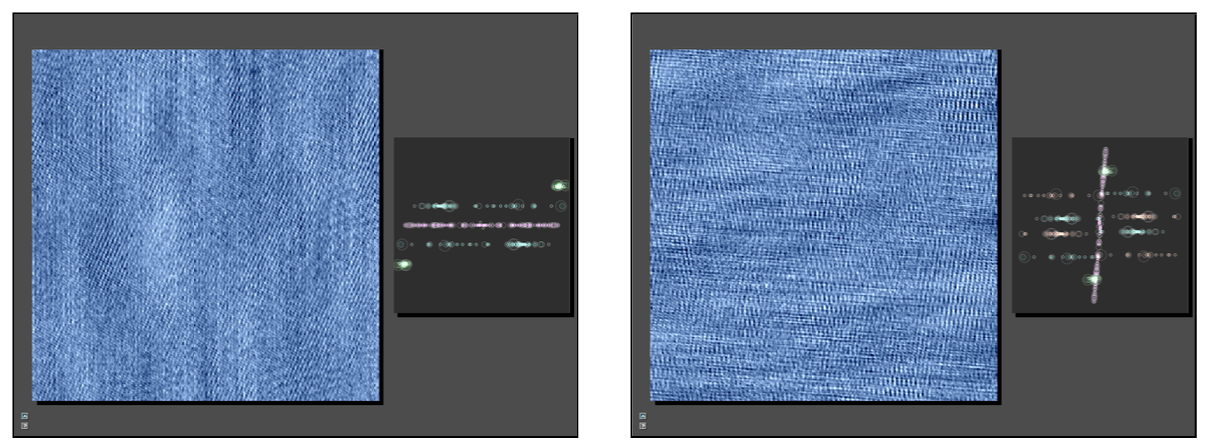
\includegraphics[width=\linewidth]{figures/analysis/galerne_2012_gne.png}}
    \caption{\label{fig:galerne_2012_gne}In blue, Gabor noise examples. To their right an interactive visualization of their power spectrum for editing the visual characteristics.~\cite{galerne_2012_gne}.}
\end{figure}

\paragraph*{Example-Based}
\label{para:analysis_stochastic_examplebased_control}

\rev{Condensing}{

Most example-based stochastic texturing techniques do not offer further artist input beyond the exemplar but focus on performance. \citeauthor*{lagae_2010_pis}~\cite{lagae_2010_pis} match noise bandwidth for isotropic multi-resolution noise in a few milliseconds, given by \citeauthor*{gilet_2012_mkn}~\cite{gilet_2012_mkn}. \citeauthor*{galerne_2017_tno}~\cite{galerne_2017_tno} introduced an efficient sparse convolution noise based on textons. The example match takes between half a second and five seconds, depending on the resolution.

\citeauthor*{galerne_2012_gne}~\cite{galerne_2012_gne} add to the example fitting an interactive visual editor for adjusting their Gabor noise, taking about two minutes per texture,. Sets of Gaussians represent the power spectrum of the noise, which can be rotated, scaled, translated, and cloned. Due to the abstract visual nature of a power spectrum, its connection to the visual features of the noise is not directly intuitive for artists. Hence, the editor has a strong exploratory nature to it. However, as the editing itself is interactive and visually appealing, it is inviting to do so. 

\citeauthor*{gilet_2012_mkn}~\cite{gilet_2012_mkn} focus on increasing the expressiveness of their model toward more structural texture designs. For that, they introduce a noise that can approximate arbitrary spectral energy distributions. A straightforward noise-by-example computation takes up to 20 seconds, depending on the number of artist-defined convolution noises. For greater control and expressiveness, a perturbation function and a multi-layer approach are presented and some configurations can be given by artist-defined image maps. Further pursuing the topic of greater expressiveness and structured noise, \citeauthor*{gilet_2014_lrn}~\cite{gilet_2014_lrn} introduced a local random phase noise. Adjustable parameters control the visual quality of the noise and the amount of structure in comparison to noise. The authors do not report performance times for the matching step. \citeauthor*{pavie_2016_pts}~\cite{pavie_2016_pts} argue for control mechanisms being more intuitive in the spatial domain instead of the commonly-used editing of the power spectrum and align local random phase noise on a regular grid with a spot noise model based on a random distribution of structured kernels. Artists have interactive control of the spatial structures by modifying the spot functions and their distribution, thus increasing the range of possible designs.

\citeauthor*{guingo_2017_btm}~\cite{guingo_2017_btm} further improve on spatial variation and visual quality. They base their work on an underlying novel noise model and separate the handling of structures. Artists need to configure the fitting, and the performance of matching a $512\times512$ input image can take up to one hour with the current implementation not parallelized. \citeauthor*{kang_2017_fpt}~\cite{kang_2017_fpt} combine procedural noise with a data-driven tiling. So-called ``non-features'' are obtained by a noise-by-example method. ``Features'' such as edges can be edited in the feature image and are combined with the noise based on an artist-controlled ratio. The feature extraction for a $257\times257$ input image, and therefore the texture matching, ranges from few seconds to two minutes. \citeauthor*{gilet_2010_ias}~\cite{gilet_2010_ias} apply a more general optimization strategy for choosing the parameters of a noise-based model. With a given estimated light source direction in the input, \citeauthor*{gilet_2010_ias}~\cite{gilet_2010_ias} can create displacement map textures, with the parameter computation taking from one to three hours. With a given rough approximation of the geometry and a representative pattern patch in the input, even volumetric representations can be created from the exemplar.}

% \rev{High-level descripton}{Overall, example-based techniques that focus on purely noise-based patterns have achieved interactive performance and a high level of visual details in the noise. In recent years, work explores how to expand the noise-based design space, often with a trade-off in performance.}


\subsubsection{Regular to Near-Regular Patterns}
\label{subsubsec:analysis_distribution_and_repetition_regular}

All the above discussed noise-based methods control a single stochastic procedural model. Even though recent advances greatly increase their expressiveness, the design space of noise-based models is too limited for creative pattern generation. Procedural models featuring regular to near-regular pattern designs (for a definition of the texture spectrum see \citeauthor{lin_2006_qeo}~\cite{lin_2006_qeo}) are usually optimized for specific design goals or even support a variety of procedural models within this class of designs. \Cref{fig:textures} shows several regular to near-regular patterns.

\begin{figure}[H]
    \centering
    \revimage{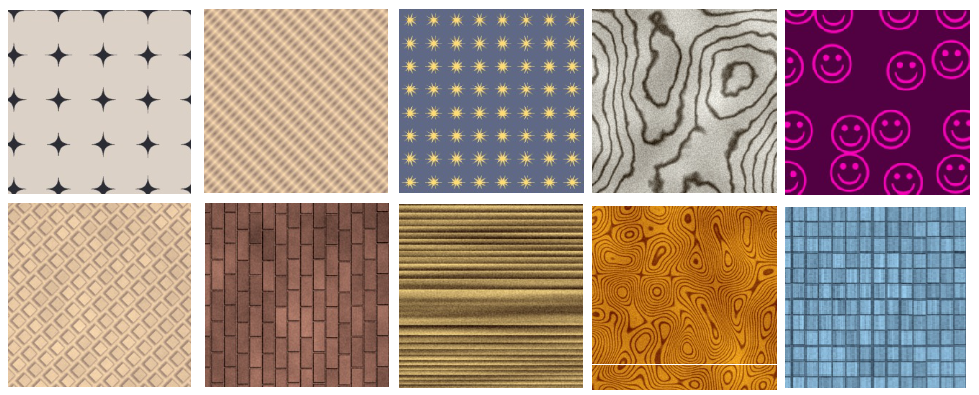
\includegraphics[width=\linewidth]{figures/analysis/textures.png}}
    \caption{\label{fig:textures}Visual examples for regular to near-regular pattern designs~\cite{gieseke_2014_ipr}.}
\end{figure}

\paragraph*{Example-Based}
\label{para:analysis_regular_example}

\rev{Condensing}{

For brick and wood textures, the early work of \citeauthor*{lefebvre_2000_ass}~\cite{lefebvre_2000_ass} presents example-based control by transferring specific measured properties of an input to corresponding parameters for the procedural representation. The authors describe the matching performance as taking from a few minutes up to an hour. Expanding the design range notably, \citeauthor{gilet_2012_map}~\cite{gilet_2012_map} focus on the interactive creation of procedural semi-structured texture models and their visual features. Random variations of artist input pattern are generated considering hierarchical spatial relationships, . In order to do so, an artist needs to give multiple exemplary object distributions. 

\citeauthor*{bourque_2004_ptm}~\cite{bourque_2004_ptm} allow for the whole procedural texture spectrum with a parameter retrieval technique. For the fitting, artists need to chose a configuration from two types of similarity metrics and two types of optimization strategies. As initialization for the optimization, the authors propose ``on the order of 200'' pre-computed random choices. The authors report an average optimization time of 12 minutes, not specifying for how many parameters. However, \citeauthor*{gilet_2012_mkn}~\cite{gilet_2012_mkn} report more than an hour runtime. With a higher number of parameters the current form of the approach quickly becomes unfeasible. \citeauthor*{gieseke_2014_ipr}~\cite{gieseke_2014_ipr} build up on the work of \citeauthor*{bourque_2004_ptm}~\cite{bourque_2004_ptm} and interpret the parameter matching as retrieval task. Based on pre-computed caches and a perceptually motivated image metric, their technique achieves interactive performance for fitting a $256\times256$ exemplar. As a one time investment the caches for the textures have to be computed. An artist has to chose the texture model to be matched. A similar approach offer \citeauthor*{hu_2019_anf}~\cite{hu_2019_anf} by training convolutional neural networks for the parameter retrieval. A style transfer step in the pixel domain is added for fitting visual details. Next to the given input example, the user has to chose from four high level texture classes. With the pre-computed caches ready, the fitting is interactive, with performances around one second, depending on texture resolution. The style-transfer lies in the range of minutes.} \rev{High level descripton}{Overall, for parameter retrieval methods the parameter count is highly influential on the performance for both visual quality and computation time. Heavy one-time investments must be made to compute the caches or train the network, which then determine the possible design spaces. Artists could use such techniques for computing a reasonable starting point for their creative work.}

\rev{Condensing and contextualization}{
While focusing on stochastic pattern, the semi-procedural approach of \citeauthor*{guehl_2020_stu}~\cite{guehl_2020_stu} offer a much larger design space than related methods by enabling the combination of patterns. The technique generates textures based on input exemplars and gives an artist the option for manual editing and database browsing to shape the output (\Cref{fig:guehl_2020_stu})
% \mfcomment{non-monotonic Figure ordering: if the Figure is referenced here, it should probably come before Figure 6, which is first reference in 7.1.3 below.}\pa{Yes, I agree 100\%. Please move the figure here.}.
At its core the system is based on a noise-by-example approach. The appearance space of the noise can be explored with an interactive 2D map and the browsing of a database of preview images, which are unusual options for example-based modeling. The interactive 2D map is visually abstract and not suitable for reaching a specific output quickly but helpful for exploring the design space. Data-driven details are smoothly combined with the noise and the user can adjust the output with different parameters. The system is interactive with reported synthesis times below one second.}


\begin{figure}[H]
    \centering
    \revimage{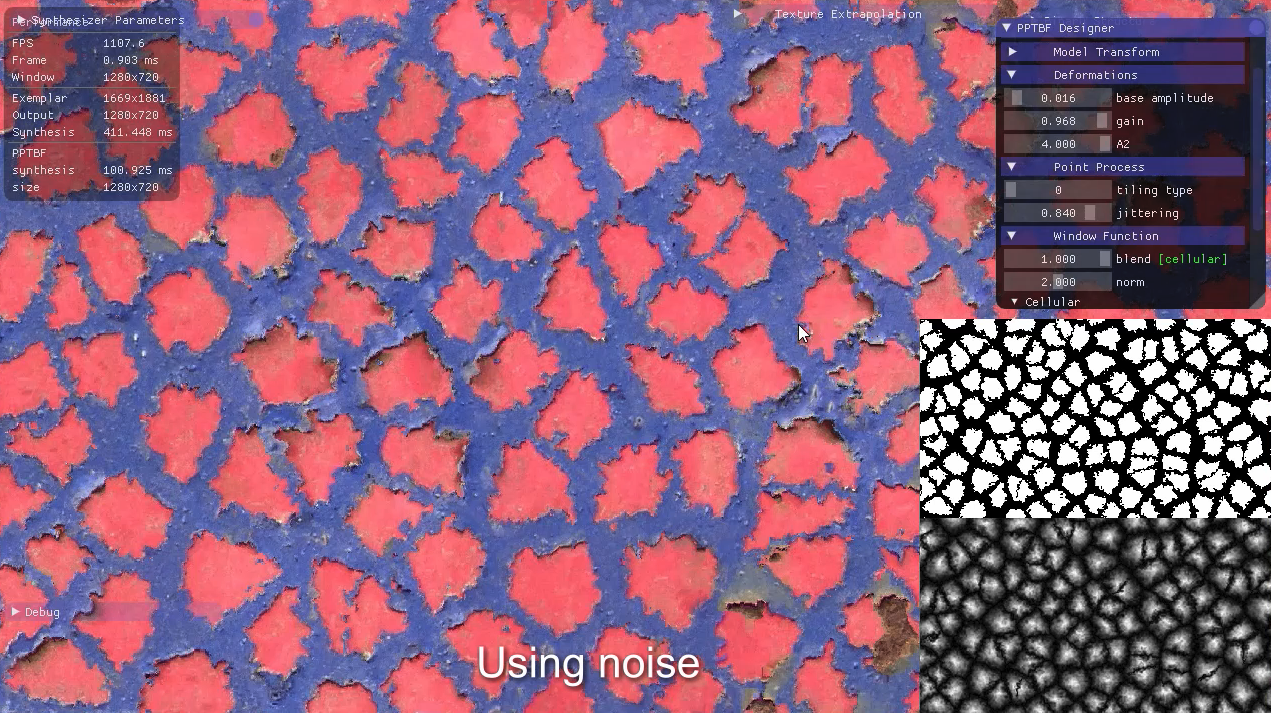
\includegraphics[width=\linewidth]{figures/discussion/guehl_2020_stu.png}}
    \caption{\label{fig:guehl_2020_stu}\citeauthor*{guehl_2020_stu}~\cite{guehl_2020_stu} offer various control mechanisms for a semi-procedural generation of stochastic patterns (examples from the supplemental video). With the different controls, an artist can work explorative as well as implement a specific design goal efficiently. }
\end{figure}


\subparagraph*{Data-Driven}
\label{subpara:analysis_regular_tilings}

\rev{Added reference, review 5}{By adding appearance as an objective when optimizing for a structurally sound topology, \citeauthor*{martinez_2015_saa}~\cite{martinez_2015_saa} offer a data-driven example-based approach. Example patterns are given as raster images. The authors report on performances between 1 and 15 minutes for exemplars up to 330$\times$330.} \rev{Condensing}{\citeauthor*{bian_2018_tpd}~\cite{bian_2018_tpd} build upon that work by controlling topology appearance with custom-made vector pattern tilings. The technique is worth pointing out for automatically helping an artist create structurally sound connections between manually drawn tiles. Tiles can be drawn from scratch. The interactive interface gives hints and corrections for the construction of structurally sound designs, such as previews of the pattern on the canvas, snapping to proper correction points, and automatic corrections near tile boundaries. Similarly,~\citeauthor*{li_2019_aqp}~\cite{li_2019_aqp} optimize for structural soundness when putting decorative elements together to generate quilting patterns. A user inputs the decorative element, a region boundary and configuration values. Then a quilting pattern is generated automatically. There are no further adjustments of the result possible. The performance is below ten seconds.

Similar to the interactive authoring of~\citeauthor*{bian_2018_tpd}~\cite{bian_2018_tpd}, \citeauthor*{tu_2020_cct}~\cite{tu_2020_cct} merge automation with manual creation. The algorithm synthesizes continuous curve patterns from exemplars made of Bézier curves, replicating not only on the position of the elements but also on their connectivity. The authors report matching times of 160 seconds depending on the sampling density. The example-based generation process is supported by various artist-controllable interactions before, during and after the creation process. Connections are continuously re-computed. An artist can also draw the example and connections directly on the canvas from scratch.}

\citeauthor*{zehnder_2016_dso}~\cite{zehnder_2016_dso} provide artists with a tool to directly assemble structurally sound curve networks on a three-dimensional surface in 3D. The components of the network are spline curves defined by the artist. Components can be placed manually or are repeated semi-automatically. The curves can be moved on the surface while having an elastic quality to them, which seems to be a quite engaging task. To prevent structural weaknesses, the system indicates problematic areas and suggests improvements, seamlessly combining the design task with engineering requirements. The performance of the automatic packing highly depends in the number of curves and ranges from seconds up to 15 minutes on average for the presented examples. For filigrees, which are thinly structured repetitive patterns, \citeauthor*{chen_2016_sof}~\cite{chen_2016_sof} present a mainly data-driven approach. \rev{Condensing}{Their method automatically distributes and assembles a set of suitable input elements. The filigrees are mechanically strengthened through the optimization of a packing problem, which must be configured by the artist. Additionally, a directional stroke field can be drawn on the canvas, controlling element orientation and size. Element distribution percentages can be given when multiple elements are combined into one common pattern. The performance in two-dimensional space runs from 6 to 26 seconds.}


\rev{High-level descripton}{Within their specific design spaces, the example-based data-driven techniques of \citeauthor*{bian_2018_tpd}~\cite{bian_2018_tpd}, \citeauthor*{tu_2020_cct}~\cite{tu_2020_cct}, and \citeauthor*{zehnder_2016_dso}~\cite{zehnder_2016_dso} highlight the promising direction of automating filling and repetition, and computing, \eg structural constraints, while giving an artist enough interactivity for creative exploration.}


\subsubsection{Rule-based and Design-Specific Patterns}
\label{subsubsec:analysis_rulebased_and_designspecific}

In the following we summarize designs that are based on a specific set of rules or grammars, as for example the ornamental patterns shown in~\Cref{fig:wong_1998_cgf} or the tangles pattern in~\Cref{fig:santoni_2016_ggp}. Hence, there are no limits to their expressiveness other than their underlying creation logic. Also, the following section discusses techniques that focus on the filling of global \textit{shapes} and \textit{masks}.

\begin{figure}[H]
    \centering
    \revimage{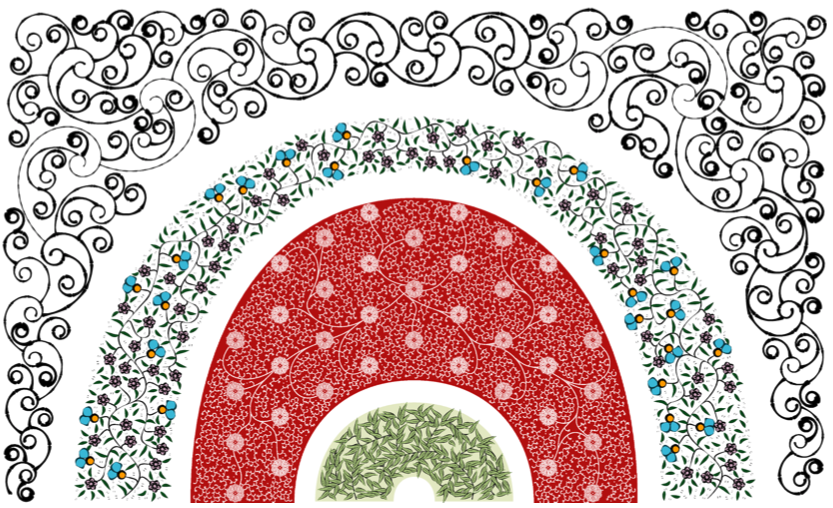
\includegraphics[width=\linewidth]{figures/analysis/wong_1998_cgf.png}}
    \caption{\label{fig:wong_1998_cgf}Visual examples for the rule-based iterative space filling model from~\citeauthor*{wong_1998_cgf}~\cite{wong_1998_cgf}.\color{orange}{Status rights: ACM requested.}}
\end{figure}


% Rule-based
\citeauthor*{wong_1998_cgf}~\cite{wong_1998_cgf} introduced a programmable procedural system that employs a greedy rule-based strategy to generate ornamental patterns. A procedural model is created with decorative elements and with a set of growth rules that handle the selection, appearance and connections of the elements. The process iterates, finding tentative places for elements by testing them against constraints in the procedural model and, where suitable, placing elements in the found spaces, optionally connecting them to existing elements. Possible ornament designs are technically restricted only by this iterative creation logic. All adjustments to the design and layout of an ornament have to be done by writing code. The authors do not report any performance times.

\rev{Higher-level, reference moved}{
\citeauthor*{santoni_2016_ggp}~\cite{santoni_2016_ggp} and \citeauthor*{gieseke_2017_ooo}~\cite{gieseke_2017_ooo} present rule-based and design specific patterns. These techniques feature frames and hierarchies and are discussed in \Cref{subsec:analysis_frames_and_hierarchies}).}  \citeauthor*{loi_2017_pae}~\cite{loi_2017_pae} present a custom-made procedural framework that can create a large variety of element texture designs. The authors aim for designs that are unrelated to their spatial location and the space they fill, calling it stationary. Their programmable method is developed for technical artists and requires programming expertise. Pattern scripts are built with partitioning, mapping and merging operators. These operators enable both global and local design control and the composition of designs. The operator-based technique would enable a node-based interface design, which is not explicitly demonstrated in the article. The execution time for most designs is a few seconds, with some examples taking more than 1 minute. A user study with technical artists carefully evaluates the system's scripting interface, concluding positive results overall.

\paragraph*{Probabilistic Interference}
\label{para:analysis_rulebased_shapes_probabilistic}

Other systems provide the control to fill an outlining shape by interpreting the procedural modeling task as a probabilistic inference problem.

\rev{Condensing and Higher-Level}{
\citeauthor*{talton_2011_mpm}~\cite{talton_2011_mpm} extend grammar-based procedural models by decoupling the growth control from the grammar itself. Their flexible analytic objective functions take images and volumes as global controls. The authors discuss that some experimentation might be needed to achieve a desired design goal, making the approach less transparent. Performance depends on the complexity of the grammar and the number of optimization steps needed. The authors report performance times ranging from a few seconds to several hours. For their examples, the authors manually terminated the optimization iteration. Similarly, \citeauthor*{ritchie_2015_cpm}~\cite{ritchie_2015_cpm} control rule-based hierarchical and iterative procedural models with image-based matching and target volumes. The work improves convergence behavior and final scores. The reported performances range from around 3 seconds to 12 minutes, and the authors show that the number of included primitives scales reasonably. \citeauthor*{ritchie_2016_ngp}~\cite{ritchie_2016_ngp} uses machine learning to improve the performance even further, increasing performance up to 10 times by integrating a neural network and sampling a learned constraint-satisfying approximation. Reported performances are overall below 3 seconds. As interactive performance is the foundation of creative control, this is of great importance.}


\paragraph*{Fields}
\label{para:analysis_rulebased_fields}

\rev{Higher-Level}{Fields have been used to creatively control the appearance of patterns with great success for several design features, meriting a separate discussion of them as control mechanisms in \Cref*{subsubsec:analysis_creative_means_fields}. In the present context, for repeating structures and filling shapes,}  \citeauthor*{yuanyuan_2011_gso}~\cite{yuanyuan_2011_gso} present a shape grammar that is guided by either a vector or tensor field. The field can influence the grammar's translation command, potentially leading to globally pronounced structures. The field can furthermore guide rotation, scaling, and color parameters. The artist can specify a priori field constraints, such as regular and singular field elements, on the surface to be filled. Once the field is computed, local Laplacian smoothing can be applied. The authors report a synthesis performance for geometric surfaces from less than a second up to 3 minutes. \rev{Added reference, review 5}{Recently, applying a parameter field and a density field for controlling the appearance, \citeauthor*{etienne_2020_pbp}~\cite{etienne_2020_pbp} present the procedural generation of band patterns as pixel shader in realtime. Both fields can be controlled by image input.}


\paragraph*{Example-Based}
\label{para:analysis_rulebased_example}

\citeauthor*{stava_2010_ipm}~\cite{stava_2010_ipm} present a context-free L-System that is able to recreate a given two-dimensional vector image consisting of groups of line segments. The algorithm creates similarity groups of these basic elements, computes spatial relationship clusters and iteratively translates these into rules. An artist is required to define a similarity threshold and significance weights for the different clusters, such as element distance or similarity, for example, thus guiding their representation according to the L-system rules. The time needed for the inverse step, depending on the number of elements in the input, is reported to range from a few seconds up to 20 minutes. \citeauthor*{talton_2012_ldp}~\cite{talton_2012_ldp} further generalize the idea of inverse grammar generation and interpret it as a probabilistic interference problem. Their system induces a probabilistic formal grammar from a hierarchy of labeled components. The authors demonstrate their technique on scene graphs for geometry models as well as DOM trees for web layouts. The authors do not report any performance times for learning design patterns.


\subsubsection{Element Arrangements}
\label{subsubsec:analysis_element_arrangements}

Element arrangements, \rev{Visual Reference}{such as shown in~\Cref{fig:ma_2011_det},} have individual and unconnected visual entities as their smallest unit. The elements themselves usually come from separate input data, such as vector graphics. In its broadest sense, the underlying distribution models for the arrangements can be seen as a procedural model. Even though there are no generative rules, characteristics of the discrete elements and their distribution can often be parametrized, and changes can be automatically processed and reproduced in the output. When filling a shape with elements or masking areas on the canvas, elements should ideally not be cut and align themselves for evenly filling the shape.
% Because many visually complex pattern contain areas of formal arranged elements, this is a relevant sub-goal for a creative pattern generation task.

\begin{figure}[htb!]
    \centering
    \revimage{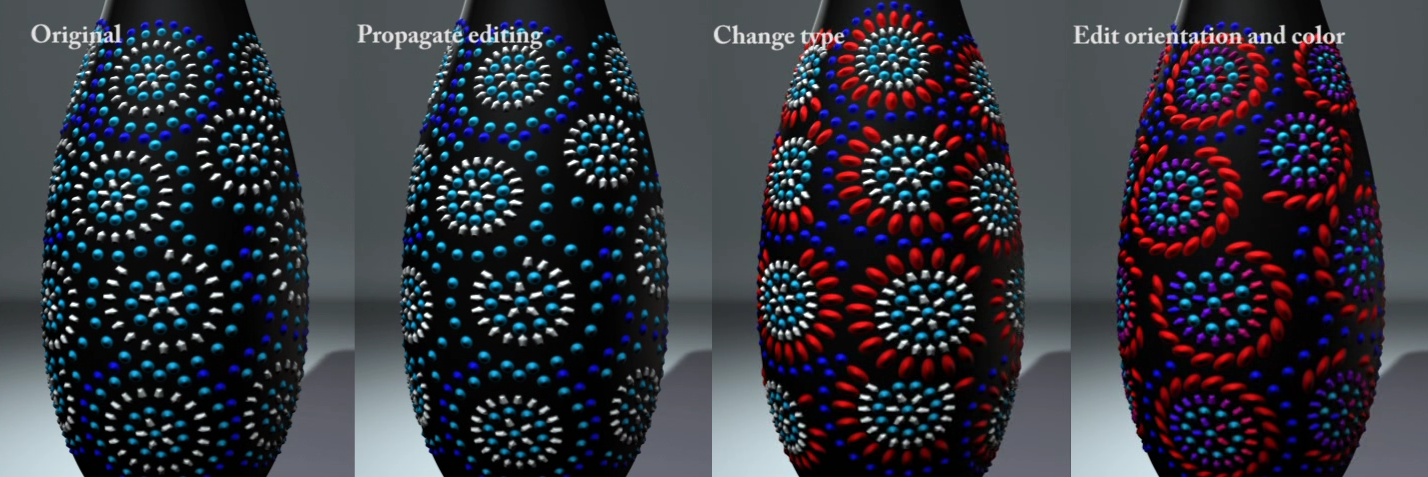
\includegraphics[width=\linewidth]{figures/analysis/ma_2011_det.png}}
    \caption{\label{fig:ma_2011_det}An example for a pattern in 3D made of discrete elements~\cite{ma_2011_det}. \citeauthor*{ma_2011_det} also offer extensive editing options such as the propagation of the edit of a single element to the overall pattern. \color{orange}{Status rights: requested}}
\end{figure}

\paragraph*{Example-Based}
\label{para:analysis_element_arrangements_example}

\rev{Higher-Level}{For an example-based generation of element arrangements, relationships between elements are usually extracted from example arrangements and reproduced for the synthesis. In the following, we only include techniques with some form of user input beyond non-creative system configuration parameters. Much previous work~\cite{peihan_2019_pps, chen_2019_mpc} focuses mainly on point distributions.}

\rev{Condensing and Higher-Level}{
 \citeauthor*{barla_2006_spa}~\cite{barla_2006_spa} and \citeauthor*{hurtut_2009_ags}~\cite{hurtut_2009_ags} focus on example-based element arrangements of stroke-based vector elements. \citeauthor*{barla_2006_spa}~\cite{barla_2006_spa} synthesize arrangements by matching local neighborhoods to a global seed distribution computed by Lloyd relaxation. Computing arrangements takes up to 10 seconds, and artist input is used in addition to the stroke patterns. Further visual adjustments are possible in a post-processing step. \citeauthor*{hurtut_2009_ags}~\cite{hurtut_2009_ags} can capture non-uniform distributions and improve the performance to the order of seconds. As a possible artist input, one exemplary shape input and density map are shown, and other input options are discussed in principle. The authors clearly state their focus to be on automation.

\citeauthor*{ijiri_2008_aeb}~\cite{ijiri_2008_aeb} combine data-driven texture synthesis with procedural generation. Their technique analyzes a given element distribution with local neighborhood comparisons and synthesizes new arrangements with interactive performance with incremental rule-based local growth. Element attributes that go beyond the positions of the elements and orientation cannot be controlled. Artists have a variety of design options with element orientation modes, an interactive spray tool to define areas to grow in, and a flow field tool to define overall alignments and a boundary tool. Moreover, the reconstructed topology can manually be adjusted. \citeauthor*{ijiri_2008_aeb}~\cite{ijiri_2008_aeb}s' work is an early example for combining a data-driven with a procedural approach. Their tools allow artists to work on the canvas directly and to focus on the actual output, even with procedural models.}

The technique of \citeauthor*{ma_2011_det}~\cite{ma_2011_det} is based on a sample of a discrete element distribution and an output shape to fill both in two and three dimensions. The exemplar has to contain the actual elements in their domain and cannot be pixel data. In order to fill the output shape with elements, an energy optimization is processed with a novel neighborhood similarity metric. In addition to element positions, the metric includes variable features referring to orientation, geometry, appearance and type, for example. Hence, the metric is capable of reproducing global aggregate distributions that go beyond local element placements. The authors also extended their work to the spatial-temporal domain~\cite{ma_2013_det}. Necessary inputs are the exemplary element distribution, the neighborhood size to consider and the output shape. Further distribution constraints based on element attributes are optional. Examples for the inclusion of a vector field and element drag and drop are given. The authors report performance times between one and ten minutes with a non-optimized implementation.

\rev{Higher-Level}{
\citeauthor*{almeraj_2013_pgt}~\cite{almeraj_2013_pgt} base their example-based geometric texture generation technique on how such textures were manually created in a previous user study~\cite{almeraj_2011_tgt}. The idea of developing a generation algorithm based on a systematic study of how artists manually create patterns is worth further investigation. The authors identify tiling, structure and randomness as the prominently used creation strategies. The patch-based algorithm, which focuses on eliminating the appearance of regularity, doesn't seem to allow for any user interaction. The authors do not report on the performance.}\rev{Condensing}{ \citeauthor*{landes_2013_asm}~\cite{landes_2013_asm} present an element distribution technique in 2D as well as 3D that improves on collision-free and anisotropic distributions with spatial relationship measurements.} Next to the exemplar, there are several user inputs possible, such as a gradient image for the distribution intensity and parameter for the fitting algorithm. Even though these can control a visual range, their communication is quite abstract. Performances range from seconds to several minutes depending on the complexity of the arrangement.


\paragraph*{Fields}
\label{para:analysis_element_arrangements_fields}

\citeauthor*{saputra_2017_ffo}~\cite{saputra_2017_ffo} optimize a flow-based ornamental packing of elements into a two-dimensional outline. For each element, a predefined spine controls the element's deformation. The artist defines direction guides and optionally fixed elements that control the computation of evenly placed streamlines. Elements are placed and deformed along streamlines. An iterative refinement step optimizes for a dense and balanced filling. An average packing takes about an hour. \citeauthor*{saputra_2018_rde}~\cite{saputra_2018_rde} build up on their previous work substituting the flow-based packing with a mass-spring system. An additional secondary packing step further fills gaps with simpler shapes. With that the technique achieves denser and more even packings. A user provides primary and optionally secondary elements, the closed shape to fill and a distance for the spacing between elements. Packings take between 2 to 20 minutes, including both, the packing of the primary and secondary elements.

\citeauthor*{hsu_2020_aef}~\cite{hsu_2020_aef} present an interactive brushing systems for placing aggregations of elements directly. As the work stands out through its brush-based control mechanisms, we discuss it in \Cref{subsec:analysis_curves}.


\paragraph*{Data-Driven}
\label{para:analysis_element_arrangements_datadriven}

\citeauthor*{phan_2016_ple}~\cite{phan_2016_ple} offer a data-driven recommendation system for circular ornamentation, employing a machine-learned style and composition feature vector. Based on a custom ring-based layout system that represents, for example, plates and vases and a first decorative element chosen by the artist, the system completes a design. The artist can also chose to incrementally add elements manually, while the system accompanies this by suggesting suitable elements and placements. This work indicates the promising direction of using learned characteristics for tools that stimulate with, \eg meaningful design suggestions.


\subsection{Frames and Hierarchies}
\label{subsec:analysis_frames_and_hierarchies}

\rev{Better Explanation of Structure}{For the design feature of frames and hierarchies, results usually consist of different pattern in different areas (\Cref{fig:santoni_2016_ggp}). Frames are either based on filling a frame-shaped space or on lines and curves.} This type of control usually gives an artist more direct visual control than the previously discussed methods, which mainly focus on filling a shape. In addition to the visual output being further structured, the control is put onto the actual canvas.\rev{Better Explanation of Structure}{In the following, we cluster this work based on curves, shapes, and masks.}

\begin{figure}[H]
    \centering
    \revimage{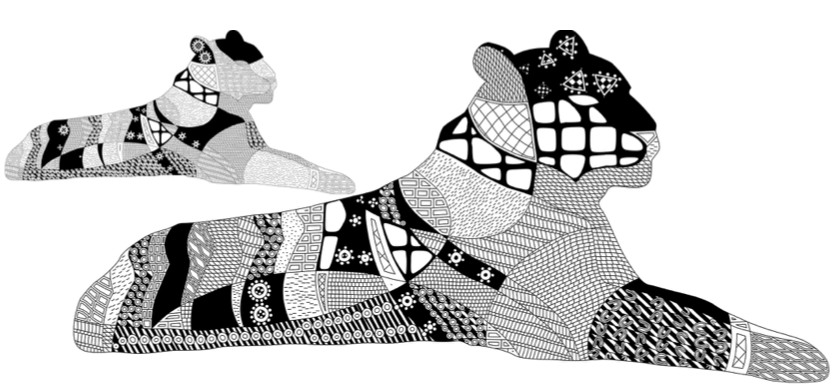
\includegraphics[width=\linewidth]{figures/analysis/santoni_2016_ggp_fig17.png}}
    \caption{\label{fig:santoni_2016_ggp}An example for a tangle pattern from \citeauthor*{santoni_2016_ggp}~\cite{santoni_2016_ggp}. On the left, the automatically generated tangle pattern and on the right the pattern is further edited by an artist.}
\end{figure}

\paragraph*{Curves} \citeauthor*{anderson_2008_udt}~\cite{anderson_2008_udt} place discrete elements on the sides of an artist-given curve based on techniques from \citeauthor*{wong_1998_cgf}~\cite{wong_1998_cgf}. \rev{Condensing}{The artist can input masks and use proxies to control the size and type of elements to be placed next to the curve. Two interfaces exist, the interactive view and the buffer view. The authors do not report a user study or specific performance times but call their system interactive. 

% Shape-based, grammar
\paragraph*{Shapes and Masks} \citeauthor*{benes_2011_gpm}~\cite{benes_2011_gpm} offer a complex shape-filling and masking system for procedural L-system models by dividing a target space into artist-editable guide shapes. Seeds for the L-system are interactively given by an artist as a position and orientation. The guide shapes determine what types of patterns grow in different areas. The connections between the shapes are manually specified by the artist and in turn guide the connections between elements, \rev{Contextulization}{possibly creating frames and emphasizing hierarchies}. Based on a mass-spring system, the guides can be intuitively edited as a whole. The authors report 30 minutes up to one hour for inferring the L-systems. The generation times for most pattern examples are less than a second, with up to 45 seconds for only one complex scenario.

% TODO: move in table and everywhere
\rev{Higher-level}{
\citeauthor*{santoni_2016_ggp}~\cite{santoni_2016_ggp} present the design-specific generation of tangles with a stochastic shape grammar. Tangles are repetitive black-and-white hand-drawn patterns made from dots, straight lines, simple curves and circles (\Cref{fig:santoni_2016_ggp}). The visual elements of Tangle patterns can align to the shape they fill and with that they can create borders, frames and hierarchies automatically. A tangle generation usually takes a few seconds, with a complex example taking about 3 minutes. The authors present an interactive system for creation based on a parameterized artist interface, including rule re-expansion and sketch-based operator modification. The presented system is a powerful combination of editing operations with procedural generation. The work also includes navigation through the editing history, which is noteworthy as this basic operation needed for creative control is usually overlooked.  A user study evaluates the system as accurate, controllable and easy to use after a reasonable training time.} 

\paragraph*{Curves, Shapes and Masks} Also building upon \citeauthor*{wong_1998_cgf}~\cite{wong_1998_cgf}, \citeauthor*{gieseke_2017_ooo}~\cite{gieseke_2017_ooo} offer, among other features, several mechanisms to create frames and hierarchies for procedural models. The authors specifically focus on the on the generation of procedural ornamentation. At the core of their system, procedural element placement can be combined with custom-made placement functions, which enable global design constraints such as symmetry. An artist can control the overall growth of the pattern as well as the connectivity of the elements by drawing frames and paths directly onto the canvas or by designing a vector field by sketching its directions. While all editing steps are interactive, more complex designs can have computation times up to several minutes, depending on the chosen placement functions.}


\subsection{Curves and Brushing}
\label{subsec:analysis_curves}

% Argue better connection between as visual element and as control element
\rev{Better Explanation of Structure}{For the design feature of curves and brushing, we consider curves and brushing as visual elements, as well as the overall control mechanism, which in turn leads to a distinct visual style. \Cref{fig:curves} give a visual example of both approaches. For brushing, we further cluster data-driven mechanisms and feature exploration techniques.} 

Formed curves such as circles, spirals or hearts are essential components for many pattern designs, including ornamentation, and are discussed first. Incorporating an artist-defined curve as the spine of a pattern, \citeauthor*{yu_2012_ans}~\cite{yu_2012_ans} use an interactive L-system to attach decorative spiral designs to the curve given by an artist. \citeauthor*{xu_2009_mcc}~\cite{xu_2009_mcc} use the space-filling algorithm of \citeauthor*{wong_1998_cgf}~\cite{wong_1998_cgf} in combination with particle tracing in simulated magnetic forces for the generation of decorative curves. Physical properties and the initialization of the particles are the parameters for designing the curves. The computation takes less than five seconds. The authors acknowledge the non-intuitive parameterization of the system and give an example timing of two minutes for finding the parameters of a specific design goal. \citeauthor*{merrell_2010_ecs}~\cite{merrell_2010_ecs} generated a set of curves in the same style of a given parametric example curve. A style is defined by local properties, such as tangents and curvatures, that are derived from a local shape analysis. The new curves are computed with a rule-based system that allows artists to interactively edit the result. Interactivity is somewhat diminished by computation times of up to minutes for a curve set. 

\begin{figure}[H]
    \centering
    \revimage{
\includegraphics[width=\linewidth]{figures/analysis/curves.png}}
    \caption{\label{fig:curves} Left, an example for curves used as control mechanism for a data-driven approach~\cite{lu_2014_dds} and on the right for procedural pattern generation~\cite{mech_2012_tdf}.}
\end{figure}

For more individual designs, brushing methods create output along curves but do so directly without taking an a priori completed curve into consideration, as if using a spray can or a brush. Brushing techniques usually include a brush diameter, hence the size of the area to be filled along the curve. \citeauthor*{mech_2012_tdf}~\cite{mech_2012_tdf} present the flexible \textit{Deco} procedural engine and examples of brushing methods for different aspects of generating procedural models, from brushing growth constraints, such as masks, to having a pattern grow along the strokes. This discussion only refers to the actual examples given by the authors. However, the engine opens up and generalizes environments for interactive control mechanisms for various types of procedural models. For the programming of decorative pattern models within the engine, helpful functionalities, such as symmetry objects and control guides, are predefined. All artist control mechanisms have interactive performance. Overall, performance mainly depends on the pattern generation scripts. The engine can load pattern codes as a dynamic library, optimizing performance. 

\rev{Contextulization, review 4}{Building up on brush-based and region-guided texture synthesis techniques such as Painting by Feature~\cite{lukac_2013_pft},} \citeauthor*{hsu_2020_aef}~\cite{hsu_2020_aef} present an interactive brushing systems for placing aggregations of elements directly. The work focuses on an even distribution and on resolving collisions. An artist can do add, erase and replace operations with the brush and also sketch a density map. The brushing is combined with an autocomplete functionality with element fields to control the automatically filled elements' alignment based on brushed directions. Filling is computed by iteratively optimizing the scale, orientation and position of the elements. Elements can be rigid or be deformed through the packing. The technique is applicable for 2D planes, 3D surfaces and 3D volumes. Performance is below 30 seconds for 2D representations. Overall, this work is a convincing combination of manual creation with automatization for creating creative element arrangements. \citeauthor*{davison_2019_ief}~\cite{davison_2019_ief} add to the work with a brushing technique that employs several example arrangements as palettes, which can be freely combined. 

More painting-like methods can be found, for example, in procedural botanical modeling \cite{anastacio_2008_spl,chen_2008_stm,palubicki_2009_sot}, procedural landscape generation~\cite{emilien_2015_wie}, as part of a procedural water color engine~\cite{diverdi_2013_ppp} or for dynamic effects~\cite{xing_2016_eit}. 

Going far beyond simple curve structures, \citeauthor*{jacobs_2018_dbe}~\cite{jacobs_2018_dbe} developed the programming and drawing environment \textit{Dynamic Brushes}, in which an artist can create individual procedural brushes for a stylus pen. General programming logic and relevant mathematical functions for creating patterns are translated into a visual programming interface. The evaluation of the system by two professional artists shows that once initial struggles to learn the system were mastered, the artists were able capture their personal analog styles with the procedural brushes. Overall, the authors and the artists open many valuable questions about the usage of current tools and about alternative approaches that seek to seamlessly blend manual and procedural creation processes. \textit{Demystified Dynamic Brushes}~\cite{li_2020_sva} expands on this by giving an artist further options, \eg~with visualizations on the canvas to investigate the linking between the procedural modelling and the visual output. Also, the creation history is recorded and can be navigated. Overall the evaluation of the system with artists indicates that a tighter bond between visual work and programming tasks make procedural modelling to artist more accessible.

\paragraph*{Data-Driven}
\label{para:analysis_curves_datadriven}

% TODO: Check move everywhere
\rev{Condensing}{
\citeauthor*{lu_2014_dds}~\cite{lu_2014_dds} create a pattern along a sketched curve with a data-driven approach. Vector pattern exemplars are placed and deformed along the curve using optimized visual soundness. For the exemplars, an artist has to define the start and end point of their spines. The artist can refine results with ``add'' and ``erase'' constraints that are drawn on the canvas. The authors report a performance of an average of eight seconds per stroke for the examples given. A related data-driven approach for synthesizing example-based vector patterns along a curve was presented by \citeauthor*{zhou_2014_tsv}~\cite{zhou_2014_tsv} in the same year. In this work, the authors focus on ensuring a structurally sound output pattern. Artists can input topological constraints, local pattern orientations and a value for variation. Once a pattern is generated, an artist can interactively adjust the underlying curve, with the pattern being updated accordingly. Generation performances are reported from below one second up to a little more than two minutes for complex models.}


% TODO: Check move everywhere
\rev{Moved from the frame section to here}{Creating textures from pen-and-ink drawings, \citeauthor*{kazi_2012_vit}~\cite{kazi_2012_vit} present a multifaceted tool, mixing data-driven and procedural modeling. Simple manually created drawings can be automatically repeated along paths, brush strokes, and can be used to fill regions. Edits of the original drawing can be propagated to all repeated elements. A user study confirms the system's usefulness to efficiently create repetitive textures while maintaining the natural workflow and artistic control of an artist. \citeauthor*{xing_2014_apr}~\cite{xing_2014_apr} build upon that work by automatically detecting and suggesting possible repetitions to the artist, aiming for a less regular, more painting-like quality. The presented system also offers various brush options and navigation tools in order to combine automation with artist control. Neither of these two articles report on performance times for the computation of the strokes and edits.}

More data-driven painting-like methods can be found, for example, for hand-drawn animations~\cite{xing_2015_aha}, creating mosaics~\cite{igarashi_2010_dde,abdrashitov_2014_msi} and data visualization~\cite{xia_2018_ddc}.


\paragraph*{Feature Exploration}
\label{para:analysis_rulebased_exploration}

Even though not a generating technique in itself, exploration is an important characteristic of a creative process. \citeauthor*{todi_2016_sse}~\cite{todi_2016_sse} present a tool for exploring common layout types with sketched input. With the method of \citeauthor*{chen_2016_msi}~\cite{chen_2016_msi}, an artist can browse a collection of texture images by sketching highly abstracted pattern features. The represented structural features of reflection, rotation, and translation symmetries adhere to important design principles for visually pleasing patterns. One could imagine a similar intuitive approach for exploring the parameter space of an ornamental procedural representation, for example.

In the context of 3D modelling, \citeauthor*{talton_2009_emw}~\cite{talton_2009_emw} investigate a collaborative 3D modeling system by crowd-sourcing possible models and feeding the results back to the system for others to explore in a structured manner. 

\subsection{Connections, Branches and Directionality}
\label{subsec:analysis_connections_branches_and_directionality}

\rev{Better Explanation of Structure}{We discuss the design feature of connections, branches and directionality in a more generally applicable manner in this section. In comparison, the above discussed work, such as~\cite{yu_2012_ans,xu_2009_mcc, merrell_2010_ecs} enable only specific branching designs.} \rev{Contextulization}{In this category, also the already discussed technique of \citeauthor*{benes_2011_gpm}~\cite{benes_2011_gpm} is to be mentioned. Even though the work focuses on structuring a space with shapes, an artist can also control the connecting points between those shapes.} \rev{Better Explanation of Structure}{In the following, for the design feature of connections, branches and directionality, we indentify the meachnism clusters of fields, example-based, and data-driven.}

\begin{figure}[H]
    \centering
    \revimage{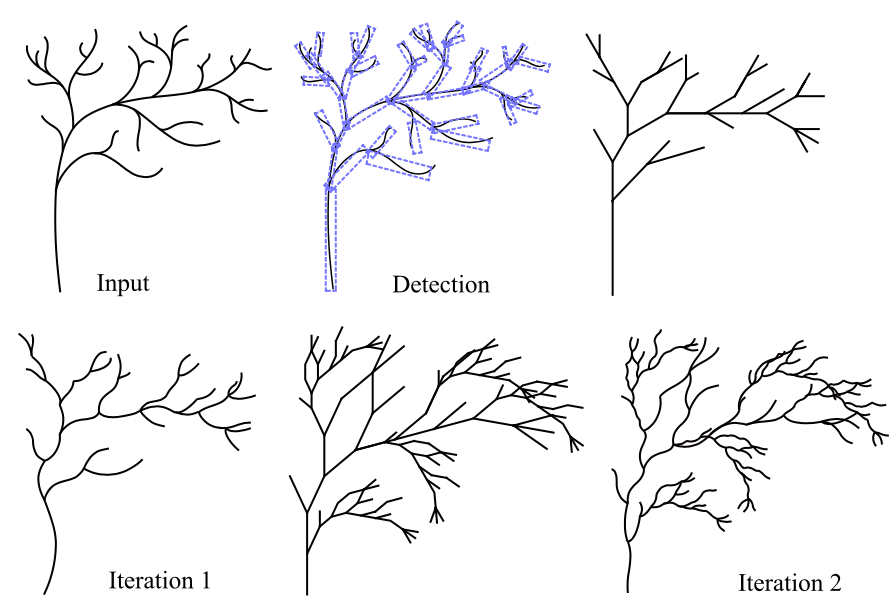
\includegraphics[width=\linewidth]{figures/analysis/guo_2020_ipm.png}}
    \caption{\label{fig:guo_2020_ipm} Visual examples for branching structures from \citeauthor*{guo_2020_ipm}~\cite{guo_2020_ipm}, who recreate a user sketch (left) with a procedural L-system (right) throug inverse modeling.\color{orange}{ Status rights: ACM request updated.}}
\end{figure}

\paragraph*{Fields}
The already discussed work of \citeauthor*{gieseke_2017_ooo}~\cite{gieseke_2017_ooo} (\Cref{subsec:analysis_frames_and_hierarchies}) enables a sense of directionality by controlling the growth of a pattern through vector fields or the connectivity and with that the branching of elements along user-specified paths. Connections between single elements can be designed through drag and drop. Also, pattern align to the space they are filling by automatically avoiding obstacles by growing around them, implemented through a shortest-path finding approach. In regard to element arrangements (\Cref{para:analysis_element_arrangements_example}), \citeauthor*{ijiri_2008_aeb}~\cite{ijiri_2008_aeb} employ vector fields to define the overall growth direction and alignment of elements within an example-guided arrangement, enabling the design of directionality. Similarly creating a sense of flow, \citeauthor*{saputra_2017_ffo}~\cite{saputra_2017_ffo} optimize a flow-based ornamental packing of elements into a two-dimensional outline. 

% TODO: Move to discussion?
Vector fields are further employed in various other specific procedural modeling contexts. For example for procedural street modeling~\cite{chen_2008_ips}, micrography~\cite{maharik_2011_dm} or botanical models~\cite{xu_2015_ptm}.

\paragraph*{Example-based}
\rev{Condensing}{\citeauthor*{guo_2020_ipm}~\cite{guo_2020_ipm} focus specifically on creating branching structures with an inverse modeling process for inferring generating L-Systems. The technique is robust and takes a variety of input designs such as real-world images or hand-drawn sketches of the branching. The inverse modeling employs convolutional neural networks, a tree graph for representing transformations and greedy optimization. Next to the exemplar, a user can input the length of the rules and the frequency of the repetition. Once the network is trained, the inference take a fraction of a second.}

\paragraph*{Data-Driven}
% Not in table.
Even though the energy-brushes of \citeauthor*{xing_2016_eit}~\cite{xing_2016_eit} are intended for creating animations (and with that not included in the table), they are easy to imagine in a pattern generation process. The technique could be used for deforming given visuals in an aesthetic manner, maybe under certain design constraints for pattern generation. With the presented brushes an artist can roughly sketch directions that shape wind, swirl, and smoke velocity fields, which in turn control the animation of the illustration. An abstracted preview of the type of brush is given on the canvas supporting an artist to translate the abstract strokes to the aspired animation. The user interface gives all basic interactions of a drawing tools, such as layers or an undo functionality. In contrast, \citeauthor*{hu_2019_ssf}~\cite{hu_2019_ssf} solve the design of velocity fields by freely sketching all possible scene elements, such as boundaries, obstacles and specific types of flow, offering more freedom but also leading to less structured results. 


\subsection{Single Accents}
\label{subsubsec:analysis_single_accents}

\rev{Better Explanation of Structure}{The design feature of single visual accents breaks with the underlying principle of procedural generation, which is to repeat certain rules and with that visual features. This overall principle is demonstrated in~\Cref{fig:guerrero_2016_pep_design}
% \mfcomment{problem: in my build, LaTeX labels this as Figure 16 and links to page 15, but it should be 11 on the same page (also 11). This indicates a problem with ordering, see,  e.g., \url{http://www.texfaq.org/FAQ-crossref} , but I do not see either the label before the caption, nor label and caption separated by different environments.}. 
However, for creative pattern generation, it is worthwhile to investigate how to combine the execution of rules with occasionally breaking such rules.  For example, \citeauthor*{gieseke_2017_ooo}~\cite{gieseke_2017_ooo} claim this to be necessary for ornamentation ``breaking an otherwise too-homogeneous appearance.'' As there is only little work somewhat matching this design feature, the are no mechanism clusters.}

Even though the required functionality can be compared to using the tip of a brush, paint-like procedural modeling techniques often have a more spray-can-like quality such as~\cite{mech_2012_tdf} and do not explicitly include the option to place one elements. \citeauthor*{gieseke_2017_ooo}~\cite{gieseke_2017_ooo} (\Cref{subsec:analysis_frames_and_hierarchies}) explicitly provide local editing options, include the deletion and placement of single elements and connections and the dragging and dropping of existing ones.

\rev{Condensing and Higher Level}{
\citeauthor*{yeh_2009_dsa}~\cite{yeh_2009_dsa} allow for separating single elements by combining a  manual data-driven design processes with procedural-modeling-like editing options. Based on detected symmetries and curvilinear element arrangements in a given vector pattern, an artist can adjust the spacing, location and scale of one element directly and propagate that change to the all other elements in the group. The authors also offer a brush that recreates recognized element groups. The technique is interactive for the examples shown but interactive performance does not scale to more complex input patterns.


\begin{figure}[H]
    \centering
    \revimage{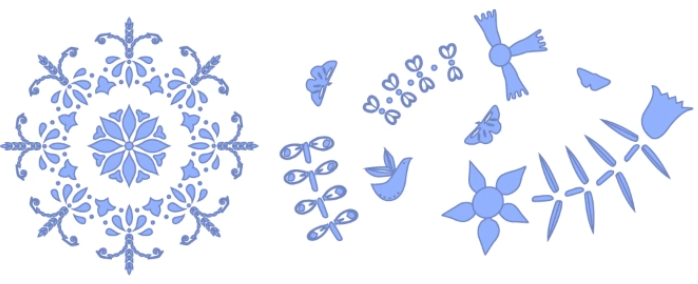
\includegraphics[width=\linewidth]{figures/analysis/guerrero_2016_pep.png}}
    \caption{\label{fig:guerrero_2016_pep_design} While the pattern exploration technique of \citeauthor*{guerrero_2016_pep}~\cite{guerrero_2016_pep} focuses on exploring design variations with repetitive visual characteristics, \eg based on symmetry, as shown on the left, the technique also enables the placement of single elements as shown on the right. Example from the supplemental video.}
\end{figure}

Also including possible single accents, the vector pattern generation technique of \citeauthor*{guerrero_2016_pep}~\cite{guerrero_2016_pep} offers suitable design variations while the artist is working on it.} An artist can select and continue with one of the offered alternatives. The system constantly re-selects from an exponential number of relevant variations based on the artist's modifications. The user interface is carefully laid out in order to offer design variations in an intuitive and efficient manner while at the same time not hindering an artist's own workflow. The authors thoroughly evaluate their system quantitatively and qualitatively - for example, with a user study. Overall, participants agreed on the usefulness of technique. 